\chapter{Systemmodelle}

\section{MVVM-Architektur}
\setcounter{counterKriterien}{0}

Es wird die MVVM-Architektur zur Realisierung von \projektTitel verwendet.

\nItem{S} Model \\
Hier befinden sich die unter Produktdatenaufgeführten punkte , Filter sowie Analysemetriken. Wenn die Daten
sich ändern schickt das Model eine Benachrichtigung an sein ViewModel.

\nItem{S} ViewModel \\
Im ViewModel werden alle vom Benutzer erhaltenen Eingaben entsprechend verarbeitet und
gegebenenfalls an das Model weitergeleitet, es leitet auch die Daten des Models and das View weiter.

\nItem{S} View \\
Ein View ist die Präsentation der Daten des Models. In unserem Fall zeigt unsere Gui den aktuellen Zusatnd des Modells.

\begin{figure}[h]
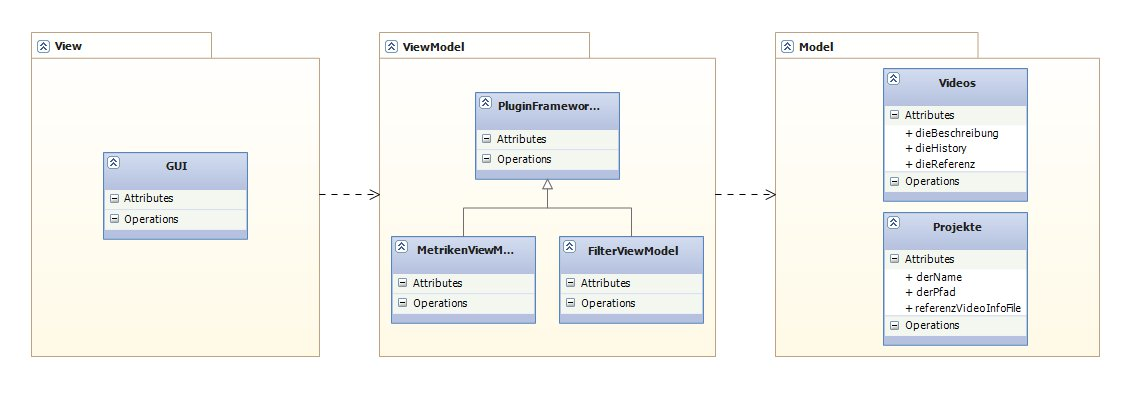
\includegraphics[width=1\linewidth]{bilder/Grobentwurf.jpg}
\label{Architektur_Grobentwurf}
\caption{Architektur-Klassendiagramm des Grobentwurfs}
\end{figure}

% Nutzt bitte dieses template für neue Szenarien
% Haltet ein Szenario bitte kürzer als eine Seite (kompilieren-> prüfen), sonst
% läuft es über die Fußzeile hinaus. Man kann es zwar mit longtable umgehen
% aber die Ereignissflussspalte wird dann auf einer eigenen Seite gedruckt.
% Außerdem sollte ein Szenario nicht so lang sein :-).
%\begin{tabular}{p{1.55cm}|p{14cm}}
%Szenario-Name & \\ \hline
%Akteur-Instanzen & \\ \hline
%Ereignis-fluss & \begin{compactenum}[1]
%\item 
%\end{compactenum} \\
%\end{tabular}



%-------------------------------------------------------------------------------------------------------
\section{Anwendungsfälle}

\begin{figure}[h]
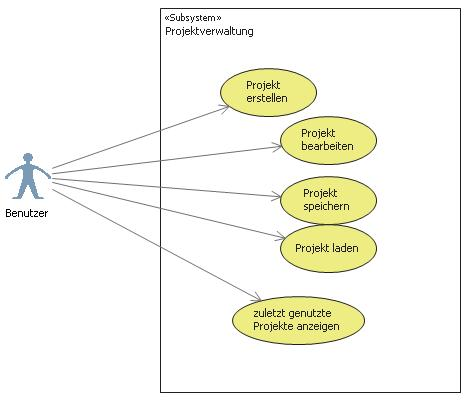
\includegraphics[scale=1]{bilder/anwendungsfalldiagramm_projektverwaltung.jpg}
\label{Anwendungsfalldiagramm_Projektverwaltung}
\caption{Anwendungsfall-Diagramm der Projektverwaltungs-Funktionalitäten}
\end{figure}

\begin{figure}[h]
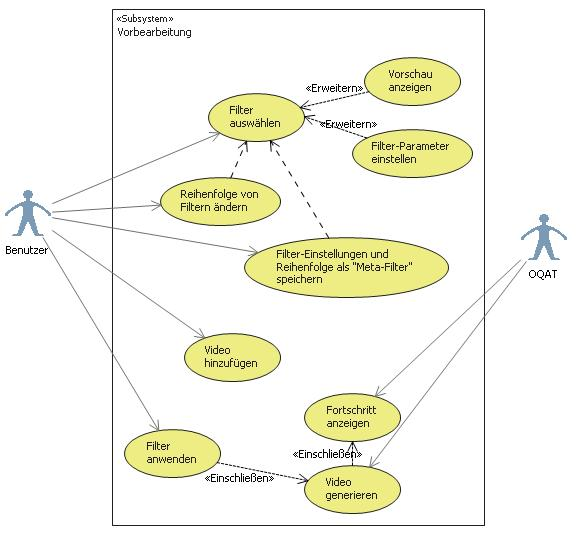
\includegraphics[scale=1]{bilder/anwendungsfalldiagramm_filter.jpg}
\label{Anwendungsfalldiagramm_Filter}
\caption{Anwendungsfall-Diagramm der Filter-Funktionalitäten}
\end{figure}

\begin{figure}[h]
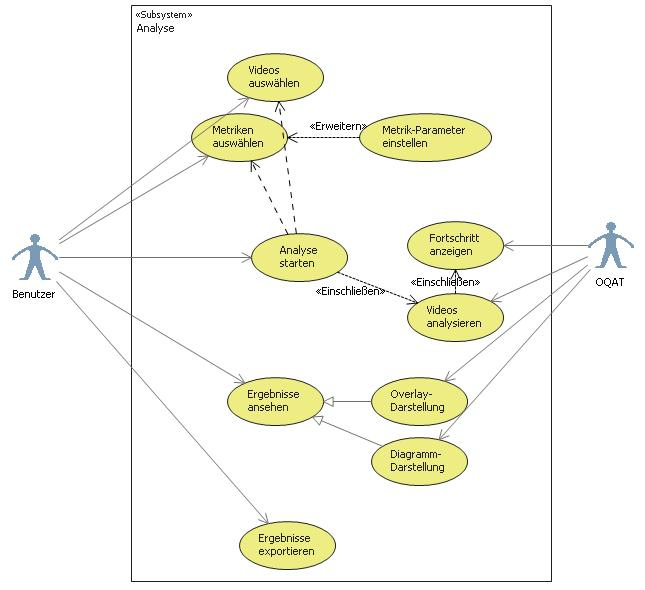
\includegraphics[scale=1]{bilder/anwendungsfalldiagramm_analyse.jpg}
\label{Anwendungsfalldiagramm_Analyse}
\caption{Anwendungsfall-Diagramm der Analyse-Funktionalitäten}
\end{figure}


% template für Anwendungsfälle, gleiche Vorschläge wie für szenario.
% Beachtet richtlinien für Anwendungsfälle (tichy oder bruegge)
%\begin{tabular}{p{2.2cm}|p{13cm}} \hline
%Anwendungs-fallname & someName\\ \hline
%Akteur & SomeActor\\ \hline
%
%Ereignisfluss & \begin{compactenum}
%\item Some process.
%\end{compactenum}\\ \hline
%
%Anfangs-bedingungen & \begin{compactitem}
%\item Some point.
%\end{compactitem} \\ \hline
%
%Abschluss-bedingungen & \begin{compactitem}
%\item Some point
%\end{compactitem}\\ \hline
%
%Qualitäts-anforderungen & \begin{compactitem}
%\item Some point
%\end{compactitem}\\ \hline
%
%\end{tabular}

%-------------------------------------------------------------------------------------------------------
